\documentclass[conference]{IEEEtran}

% Proofreading purposes.
%\documentclass[12]{article}
%\renewcommand{\baselinestretch}{2}
%\oddsidemargin 0 in
%\textwidth 7.0 in

\usepackage{graphicx}
\usepackage{psfrag}
\usepackage{subfigure}

\begin{document}

\title{Error Rate Performance in OFDM-based Cooperative Networks}

%\author{Victor~K.~Y.~Wu$^*$
%            and~Ye~(Geoffrey)~Li,~\IEEEmembership{Fellow,~IEEE}\\
%            School of Electrical and Computer Engineering \\
%            Georgia Institute of Technology \\
%            Atlanta, Georgia \\
%            Email: victor.wu@gatech.edu, liye@ece.gatech.edu
%\thanks{This work was supported by a research gift from the Nokia Research Center at Texas.}
%\thanks{*V. K. Y. Wu can be reached by telephone at (416) 512-6927 or by surface mail at 397 Ruth Avenue, North York, Ontario, Canada, M2M 2J1.}
%}

\author{\authorblockN{Victor K. Y. Wu and Ye (Geoffrey) Li}
\authorblockA{School of Electrical and Computer Engineering\\
Georgia Institute of Technology\\
Atlanta, Georgia\\
Email: vwu3@ifp.uiuc.edu, liye@ece.gatech.edu} \and
\authorblockN{Marilynn Green, Tony Reid, and Peter Wang}
\authorblockA{Nokia Siemens Networks\\
Dallas, Texas\\
Email: \{marilynn.green, tony.reid, peter.wang\}@nsn.com} }

\maketitle

\begin{abstract}
Cooperative relay networks have been shown to improve performance in wireless communication systems as a form of spatial diversity.  In this paper, we investigate the error rate performance in a single path relay network and a multiple path relay network using orthogonal frequency division multiplexing (OFDM) signals.  Using the amplify-and-forward and decode-and-forward relay algorithms, we derive input-output relations for the two networks.  For the amplify-and-forward case, we consider two relay power allocation schemes.  The first is constant gain allocation, where the amplifying gain is constant for all subcarriers.  The second is equal power allocation, where each subcarrier transmits the same power.  The former scheme does not require channel state information (CSI), while the latter one does.  For the decode-and-forward case, the transmitter and each relay are assumed to have uniform power allocations.  We simulate the word error rate (WER) performance for the two networks.  For the single path relay network, amplify-and-forward gives very poor performance, because as we increase the distance between the transmitter and receiver (and thus, add more relays), more noise and channel distortion enter the system.  Decode-and-forward gives significantly better performance because noise and channel distortion are eliminated at each relay.  For the multiple path relay network, decode-and-forward again gives better performance than amplify-and-forward.  However, the performance gains are small compared to the single path relay network case.  Therefore, amplify-and-forward may be a more attractive choice in this case due to its lower complexity.
\end{abstract}

\IEEEpeerreviewmaketitle

\section{Introduction}
\label{sec:introduction}

Recently, \emph{relays} are being exploited to improve performance
in wireless communications systems.  The relays are a network of
transceiver nodes between the transmitter and receiver that
facilitate the transfer of information. This type of scheme is
known as \emph{cooperation} or \emph{cooperative communications}
in the literature because the relay network is cooperating with
the transmitter and receiver to improve performance.  It is also
known as \emph{meshed networking}.

One current example of such technologies is the MIT-initiated One
Laptop per Child (OLPC) project \cite{website:OLPC}, which aims to
provide affordable laptops equipped with meshed networking
functionality to children in the developing world.  Since cellular
and Internet connectivity is sparse and sporadic in these regions,
such laptops can cooperate to make the best use of available
bandwidth.

In this paper, we restrict ourselves to a single path relay
network and a multiple path relay network in the context of
orthogonal frequency division multiplexing (OFDM) systems.

The authors in \cite{thesis:Laneman01}, \cite{article:Laneman01}, \cite{article:Laneman02} have provided several physical layer relay algorithms.  These include \emph{amplify-and-forward} and \emph{decode-and-forward}.  In amplify-and-forward, a node amplifies its receive symbol, subject to a power constraint, before re-transmitting to the next node.  This algorithm is obviously with low complexity.  In decode-and-forward, a node fully decodes a symbol, re-encodes it and then re-transmits it.  In other words, this scheme attempts to eliminate channel distortion and noise at each node.

The authors in \cite{article:Hasna02}, \cite{article:Hasna01} have investigated cooperation for a single path of relays connected in series.  The motivation for this network structure is that broader wireless coverage can be achieved, while still maintaining a low power constraint at the transmitter.  The authors consider \emph{analog relaying} and \emph{digital relaying} as two possible relay algorithms.  These are equivalent to the amplify-and-forward and decode-and-forward algorithms, respectively.  A power budget is considered where each packet travelling through the network is only allowed to consume a total fixed amount of power.  As well, each node has a certain transmit power limit.  The outage probability is then minimized by allocating power among the relay network under these power constraints.  This power allocation accounts for the channel conditions in the network in order to achieve the optimal outage probability.  Simulations indicate that $2$ dB of total power can be saved for 5 relays by using optimal power allocation instead of uniform power allocation.  This is for the decode-and-forward case.  However, at high $\mbox{SNR}$ values, the decode-and-forward case approximates the amplify-and-forward case.

The authors in \cite{article:Adve01} have investigated cooperation for multiple paths of relays connected in parallel.  In the conventional scheme, all relays participate using amplify-and-forward.  This is called \emph{all-participate amplify-and-forward} (AP-AF).  The authors also consider an algorithm where only one relay is selected in the transmission to maximize the mutual information.  This is called \emph{selection amplify-and-forward} (S-AF).  S-AF selects the relay which results in the maximum mutual information between transmitter and receiver.  Simulations of outage probability indicate that $5$ dB of SNR can be saved for 3 relays by using S-AF instead of AP-AF.  The authors in \cite{article:Ribeiro01} derive symbol error probabilities for multiple paths of relays.

In this paper, we continue to investigate the series and parallel cooperative relay networks using OFDM signals.  We consider a single path relay network and a multiple path relay network.  Using the amplify-and-forward relay algorithm, we derive the input-output relations for both networks.  Using a power constraint at each relay, we consider two relay power allocation schemes.  The first is constant gain allocation, where the amplifying gain is constant for all subcarriers.  The second is equal power allocation, where each subcarrier transmits the same power.  Using the decode-and-forward relay algorithm, we derive input-output relations for both networks.  We simulate word-error-rates (WERs) for the two networks using both the amplify-and-forward and decode-and-forward relay algorithms.

The paper is organized as follows.  In Section \ref{sec:sp}, we consider the single path relay network in \cite{article:Hasna02}, \cite{article:Hasna01}.  In Section \ref{sec:mp}, we consider a modified version of the multiple path relay network in \cite{article:Adve01} where the transmitter-receiver direct link is removed.  Notice that these two relay networks are series and parallel analogs of each other.  In Section \ref{sec:sr}, we present simulations of the WERs for the two relay networks.  Finally, Section \ref{sec:conclusions} concludes the paper and provides future research directions.

\section{Single Path Relay Network}
\label{sec:sp}

\begin{figure}
  \centering
    \psfrag{r0}[cc][Bl][0.8]{$r_0$}
    \psfrag{r1}[cc][Bl][0.8]{$r_1$}
    \psfrag{r3}[cc][Bl][0.8]{$r_m$}
    \psfrag{r4}[cc][Bl][0.8]{$r_{m+1}$}
    \psfrag{n0}[cc][Bl][0.8]{$n_k^{(0)}$}
    \psfrag{n2}[cc][Bl][0.8]{$n_k^{(m-1)}$}
    \psfrag{n3}[cc][Bl][0.8]{$n_k^{(m)}$}
    \psfrag{H0}[cc][Bl][0.8]{$h_k^{(0)}$}
    \psfrag{H1}[cc][Bl][0.8]{$h_k^{(1)}$}
    \psfrag{H2}[cc][Bl][0.8]{$h_k^{(m-1)}$}
    \psfrag{H3}[cc][Bl][0.8]{$h_k^{(m)}$}
    \psfrag{Tx}[cr][Bl][0.9]{Transmitter}
    \psfrag{Rx}[cl][Bl][0.9]{Receiver}
    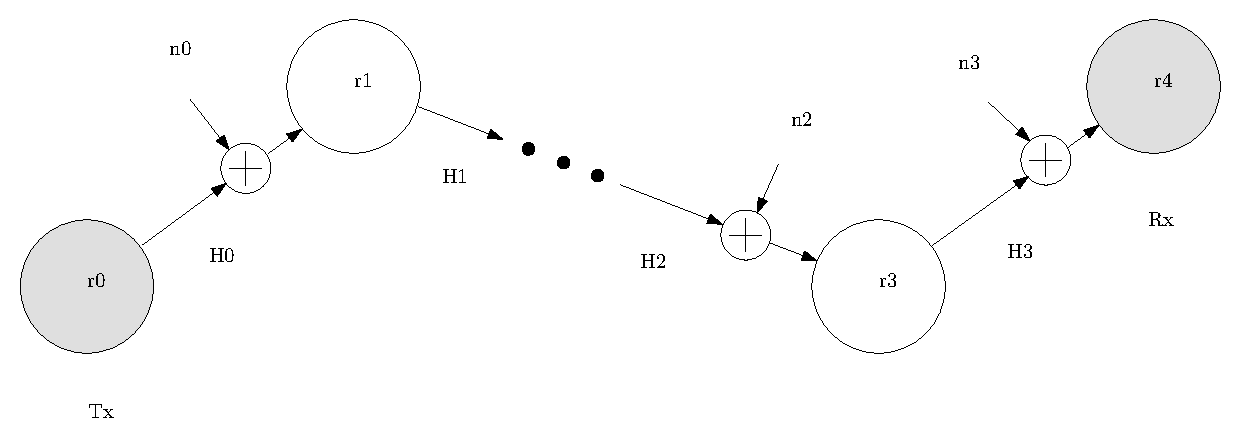
\includegraphics[width=2.5in]{sp_model.eps}
   \caption{Single Path Relay Network \label{fig:sp_sm} }
\end{figure}

\subsection{Amplify-and-Forward}
\label{sec:sp_af}
Figure \ref{fig:sp_sm} shows the single path
relay network. In the figure, $r_0$ is the transmitter, $r_{m+1}$
is the receiver, and $r_1, \ldots, r_m$ are $m$ relay nodes
connected in series forming a single path link between the
transmitter and receiver.  The relays perform amplify-and-forward
(AF) relaying. We assume that OFDM with $N$ subcarriers is used in
the system.

$h_k^{(0)}, \ldots, h_k^{(m)}$ are the complex subchannel gains at the $k^{\mbox{th}}$ subcarrier in the link, for $k = 1$ to $N$.   $n_k^{(0)}, \ldots, n_k^{(m)}$ are the corresponding noises, which are assumed to be mutually independent and circular symmetric complex Gaussians all with zero mean and variance $N_0 B / N$, where $N_0$ is the power spectral density of the underlying continuous time noise process and $B$ is the OFDM bandwidth of the system.  Let $p_k^{(0)} = P_{\mbox{tot}} / N$ be the transmit power on the $k^{\mbox{th}}$ subcarrier, where $P_{\mbox{tot}}$ is the net transmitter power.  Let  $\sqrt{p_k^{(l)}}$ be the amplifying gain used in the amplify-and-forward algorithm at the $l^{\mbox{th}}$ relay, for $l=1$ to $m$.  The $k^{\mbox{th}}$ receive symbol at $r_l$ is amplified by $\sqrt{p_k^{(l)}}$ before it is forwarded to the next node.

Let $x_k^{(0)}$ be the $k^{\mbox{th}}$ transmit symbol with zero mean and unit variance.  Let $y_k$ be the $k^{\mbox{th}}$ receive symbol at the receiver.  Let $x_k^{(l)}$ be the $k^{\mbox{th}}$ receive symbol at the $l^{\mbox{th}}$ relay.  Note that $x_k^{(l)}$ is also the $k^{\mbox{th}}$ transmit symbol at the $l^{\mbox{th}}$ relay.  Using Figure \ref{fig:sp_sm}, the input-output relation at the $l^{\mbox{th}}$ relay is
\begin{eqnarray}
x_k^{(l)} = h_k^{(l-1)} \sqrt{p_k^{(l-1)}} x_k^{(l-1)} +
n_k^{(l-1)}. \label{eqn:sp_af_inout_relay}
\end{eqnarray}
The input-output relation at the receiver is
\begin{eqnarray}
y_k = h_k^{(m)} \sqrt{p_k^{(m)}} x_k^{(m)} + n_k^{(m)}.
\label{eqn:sp_af_inout_recvr}
\end{eqnarray}
(\ref{eqn:sp_af_inout_relay}) in closed form is
\begin{eqnarray}
x_k^{(l)} = \left( \prod_{i=0}^{l-1} h_k^{(i)} \sqrt{p_k^{(i)}}
\right) x_k^{(0)} + \hspace{1.35in} \nonumber \\
\hspace{1.35in} \sum_{j=0}^{l-1} \left( \prod_{i=j+1}^{l-1}
h_k^{(i)} \sqrt{p_k^{(i)}} \right) n_k^{(j)} .
\label{eqn:sp_af_inout_relay_closed}
\end{eqnarray}
(\ref{eqn:sp_af_inout_recvr}) in closed form is
\begin{eqnarray}
y_k = \left( \prod_{i=0}^m h_k^{(i)} \sqrt{p_k^{(i)}} \right)
x_k^{(0)} + \hspace{1.35in} \nonumber \\
\hspace{1.35in} \sum_{j=0}^m \left( \prod_{i=j+1}^m h_k^{(i)}
\sqrt{p_k^{(i)}} \right) n_k^{(j)} .
\end{eqnarray}

We assume that the net transmit power at the transmitter and at each each relay is $P_{\mbox{tot}}$, that is,
\begin{eqnarray}
\sum_{k=1}^N E \left\{ \left| \sqrt{p_k^{(l)}} x_k^{(l)} \right| ^2 \right\} = P_{\mbox{tot}}.
\label{eqn:sp_af_powerconstraint_simple}
\end{eqnarray}
At the transmitter, we assume a uniform power distribution, that is, $p_k^{(0)} = P_{\mbox{tot}}/N$.  To derive the power constraint at each relay, substitute (\ref{eqn:sp_af_inout_relay_closed}) into (\ref{eqn:sp_af_powerconstraint_simple}) to arrive at
\begin{eqnarray}
\sum_{k=1}^N \frac{ p_k^{(l)}}{N} \left[
b_k^{(0)} \left( \prod_{i=1}^{l-1}  b_k^{(i)}p_k^{(i)} \right) +
\frac{1}{\mbox{SNR}} \sum_{j=0}^{l-1} \prod_{i=j+1}^{l-1}  b_k^{(i)}p_k^{(i)} \right] \nonumber \\
=1,
\label{eqn:sp_af_powerconstraint}
\end{eqnarray}
where  $b_k^{(i)} = \left| h_k^{(i)} \right|^2$, for $i=0$ to $m$ and $\mbox{SNR} = P_{\mbox{tot}} / N_0 B$.  Note that (\ref{eqn:sp_af_powerconstraint}) is defined recursively.  The power constraint for $p_k^{(l)}$ depends on $p_k^{(1)}, \dots, p_k^{(l-1)}$.  $p_k^{(1)}$ is the base case in the recursion, which follows from (\ref{eqn:sp_af_powerconstraint}), when $l = 1$.

One power allocation at the $l^{\mbox{th}}$ relay is to set $p_k^{(l)}$ constant for all subcarriers.  This results in moving $p_k^{(l)}$ in (\ref{eqn:sp_af_powerconstraint}) out of the summation because it is no longer a function of $k$
\begin{eqnarray}
p_{k,ct}^{(l)} = p_{ct}^{(l)} =  \hspace{2.35in} \nonumber \\
\frac{ N \mbox{SNR} } { \displaystyle \sum_{k=1}^N \left[
\mbox{SNR} b_k^{(0)} \left( \displaystyle \prod_{i=1}^{l-1}
b_k^{(i)} p_{ct}^{(i)}\right) + \displaystyle \sum_{j=0}^{l-1}
\displaystyle \prod_{i=j+1}^{l-1} b_k^{(i)} p_{ct}^{(i)} \right]}.
\label{eqn:sp_af_ct_allocation}
\end{eqnarray}
We call this \emph{constant gain allocation} (CT).  Note that this
power allocation does not require each relay to have any channel
state information (CSI).  That is, we do not actually need to use
(\ref{eqn:sp_af_ct_allocation}).  We can use
(\ref{eqn:sp_af_powerconstraint_simple}) directly to solve for
$p_{ct}^{(l)}$.

A second power allocation is to choose $p_k^{(l)}$ such that every subcarrier transmits the same power at the $l^{\mbox{th}}$ relay.  That is, (\ref{eqn:sp_af_powerconstraint_simple}) becomes $E \left\{ \left| \sqrt{p_{k,eq}^{(l)}} x_k^{(l)} \right| ^2 \right\} = P_{\mbox{tot}}/N$, for $k = 1$ to $N$.  This is equivalent to setting every summand on the left hand side of (\ref{eqn:sp_af_powerconstraint}) to $1/N$.  We then have
\begin{eqnarray}
p_{k,eq}^{(l)} = \frac{\mbox{SNR}}
{\mbox{SNR} b_k^{(0)} \left( \displaystyle\prod_{i=1}^{l-1}b_k^{(i)} p_{k,eq}^{(i)} \right) + \displaystyle\sum_{j=0}^{l-1}
\prod_{i=j+1}^{l-1}  b_k^{(i)} p_{k,eq}^{(i)}} \mbox{.}
\label{}
\end{eqnarray}
We call this \emph{equal power allocation} (EQ).  Note that this power allocation does require each relay to have the CSI of its upstream channels.

\subsection{Decode-and-Forward}
In decode-and-forward (DF), each relay fully recovers the information bits (with possible errors) after receiving an OFDM symbol.  It then converts the information bits back into an OFDM symbol and then transmits it.  The transmitter and all the relays transmit with the same uniform power distribution.  That is,
\begin{eqnarray}
p_k^{(0)} = p_k^{(l)} = \frac{P_{\mbox{tot}}}{N}\mbox{,}
\end{eqnarray}
for $k = 1$ to $N$ and for $l = 1$ to $m$.

Let $x_k^{(0)}$ be the $k^{\mbox{th}}$ transmit symbol from the transmitter and  $x_k^{(l)}$ be the $k^{\mbox{th}}$ transmit symbol from the $l^{\mbox{th}}$ relay, all with with zero mean and unit variance.  Let $y_k^{(m+1)}$ be the $k^{\mbox{th}}$ receive symbol at the receiver and  $y_k^{(l)}$ be the $k^{\mbox{th}}$ receive symbol at the $l^{\mbox{th}}$ relay.  Using Figure \ref{fig:sp_sm}, the input-ouput relation at the $l^{\mbox{th}}$ relay is
\begin{eqnarray}
y_k^{(l)} = h_k^{(l-1)} \sqrt{\frac{P_{\mbox{tot}}}{N}} x_k^{(l-1)} + n_k^{(l-1)} \mbox{.}
\end{eqnarray}
The input-output relation at the receiver is
\begin{eqnarray}
y_k^{(m+1)} =h_k^{(m)}  \sqrt{\frac{P_{\mbox{tot}}}{N}} x_k^{(m)} + n_k^{(m)} \mbox{.}
\end{eqnarray}

\section{Multiple Path Relay Network}
\label{sec:mp}

\begin{figure}
  \centering
    \psfrag{r0}[cc][Bl][0.8]{$r_0$}
    \psfrag{r1}[cc][Bl][0.8]{$r_1$}
    \psfrag{r3}[cc][Bl][0.8]{$r_m$}
    \psfrag{r4}[cc][Bl][0.8]{$r_{m+1}$}
    \psfrag{n01}[cc][Bl][0.8]{$n_k^{(0|1)}$}
    \psfrag{n03}[cc][Bl][0.8]{$n_k^{(0|m)}$}
    \psfrag{n14}[cc][Bl][0.8]{$n_k^{(1|m+1)}$}
    \psfrag{n34}[cc][Bl][0.8]{$n_k^{(m|m+1)}$}
    \psfrag{H01}[cc][Bl][0.8]{$h_k^{(0|1)}$}
    \psfrag{H03}[cc][Bl][0.8]{$h_k^{(0|m)}$}
    \psfrag{H14}[cc][Bl][0.8]{$h_k^{(1|m+1)}$}
    \psfrag{H34}[cc][Bl][0.8]{$h_k^{(m|m+1)}$}
    \psfrag{Tx}[cr][Bl][0.9]{Transmitter}
    \psfrag{Rx}[cl][Bl][0.9]{Receiver}
    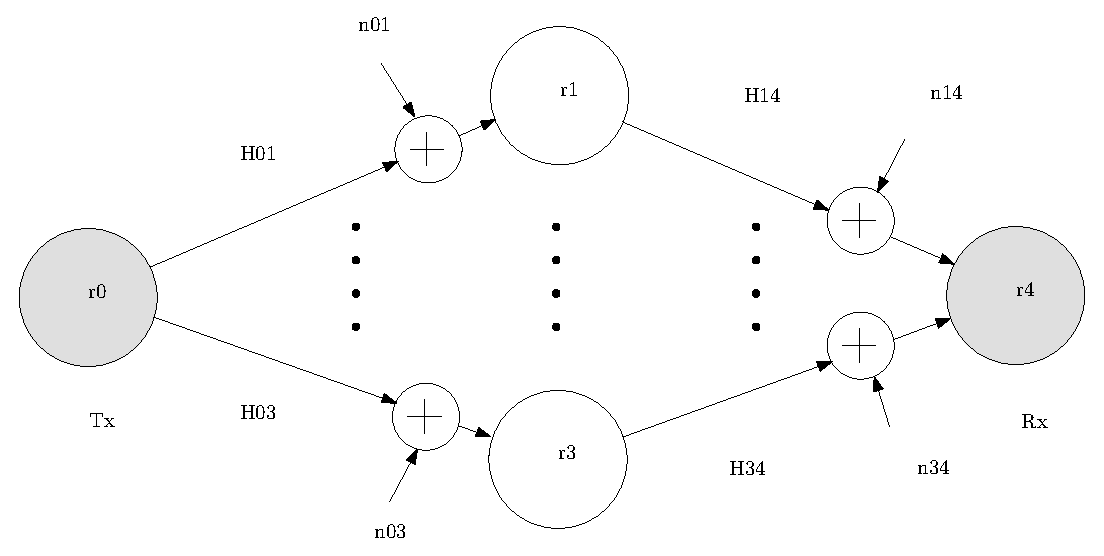
\includegraphics[width=2.5in]{mp_model.eps}
   \caption{Multiple Path Relay Network \label{fig:mp_sm} }
\end{figure}


\subsection{Amplify-and-Forward}
Figure \ref{fig:mp_sm} shows the multiple path relay network.  In the figure, $r_0$ is the transmitter, $r_{m+1}$ is the receiver, and $r_1, \ldots, r_m$ are $m$ relay nodes connected in parallel forming a multiple path link between the transmitter and receiver.  The relays perform amplify-and-forward (AF) relaying.  We assume that OFDM with $N$ subcarriers is used in the system.

$h_k^{(0|1)}, \ldots, h_k^{(0|m)}, h_k^{(1|m+1)}, \ldots, h_k^{(m|m+1)}$ are the complex subchannel gains at the $k^{\mbox{th}}$ subcarrier in the link, for $k = 1$ to $N$.   $n_k^{(0|1)}, \ldots, n_k^{(0|m)}, n_k^{(1|m+1)}, \ldots, n_k^{(m|m+1)}$ are the corresponding noises, which are assumed to be mutually independent, zero-mean, circular symmetric complex Gaussians all with variance $N_0 B / N$, where $N_0$ is the power spectral density of the underlying continuous time noise process and $B$ is the OFDM bandwidth of the system.  Let $p_k^{(0)} = P_{\mbox{tot}}/N$ be the transmitter power on the $k^{\mbox{th}}$ subcarrier, where $P_{\mbox{tot}}$ is the net transmitter power.  Let  $\sqrt{p_k^{(l)}}$ be the amplifying gain used in the amplify-and-forward algorithm at the $l^{\mbox{th}}$ relay, for $l=1$ to $m$.  The $k^{\mbox{th}}$ receive symbol at $r_l$ is amplified by $\sqrt{p_k^{(l)}}$ before it is forwarded to the next node.

Let $x_k$ be the $k^{\mbox{th}}$ transmit symbol with zero mean and unit variance.  Let $y_k^{(l)}$  be the $k^{\mbox{th}}$ receive symbol from the $l^{\mbox{th}}$ path at the receiver.  Using Figure \ref{fig:mp_sm}, the input-output relation for the $l^{\mbox{th}}$ path is
\begin{eqnarray}
y_k^{(l)} = \left( h_k^{(0|l)} h_k^{(l|m+1)} \sqrt{p_k^{(0)}} \sqrt{p_k^{(l)}} \right) x_k
+ \hspace{.75in} \nonumber \\
\hspace{.75in} h_k^{(l|m+1)} \sqrt{p_k^{(l)}}  n_k^{(0|l)} +
n_k^{(l|m+1)}. \label{eqn:mp_af_inout}
\end{eqnarray}

We assume that the net transmit power at the transmitter and at
each each relay is $P_{\mbox{tot}}$, as in
(\ref{eqn:sp_af_powerconstraint_simple}).  At the transmitter, we
assume a uniform power distribution, that is, $p_k^{(0)} =
P_{\mbox{tot}}/N$.  To derive the power constraint at each relay
and thus, possible power allocations, we use a derivation similar
to the one in Section \ref{sec:sp_af} to arrive at
\begin{eqnarray}
\sum_{k=1}^N \frac{ p_k^{(l)}}{N} \left(
b_k^{(0|l)} +
\frac{1}{\mbox{SNR}} \right) =1,
\label{eqn:mp_af_powerconstraint}
\end{eqnarray}
where $b_k^{(i|j)} = \left| h_k^{(i|j)} \right|^2$, for $i=0$ to $m$, for $j=1$ to $m+1$, $i \neq j$, and $\mbox{SNR} = P_{\mbox{tot}} / N_0 B$.

\emph{Constant gain allocation} (CT) in this case is
\begin{eqnarray}
p_{k,ct}^{(l)} = p_{ct}^{(l)} =
 \frac{N \mbox{SNR}}
{\displaystyle \sum_{k=1}^N \left( \mbox{SNR} b_k^{(0)} + 1 \right)
} \mbox{.}
\end{eqnarray}
Again, this power allocation does not require each relay to have
any channel state information (CSI).  The $l^{\mbox{th}}$ relay
only has to multiply its entire OFDM receive symbol by a constant,
$\sqrt{p_{ct}^{(l)}}$, such that the total transmit power is
$P_{\mbox{tot}}$, similar to constant gain allocation in Section
\ref{sec:sp_af}.

\emph{Equal power allocation} (EQ) in this case is
\begin{eqnarray}
p_{k,eq}^{(l)} =  \frac{ \mbox{SNR}}
{\displaystyle  \mbox{SNR} b_k^{(0|l)} + 1} \mbox{.}
\end{eqnarray}
Note that this power allocation does require each relay to have the CSI of its upstream channel.

\subsection{Decode-and-Forward}
In decode-and-forward (DF), each relay fully recovers the information bits (with possible errors) after receiving an OFDM symbol.  It then converts the information bits back into an OFDM symbol and then transmits it.  The transmitter and all the relays transmit with the same uniform power distribution.  That is,
\begin{eqnarray}
p_k^{(0)} = p_k^{(l)} = \frac{P_{\mbox{tot}}}{N}\mbox{,}
\end{eqnarray}
for $k = 1$ to $N$ and for $l = 1$ to $m$.

Let $x_k^{(0)}$ be the $k^{\mbox{th}}$ transmit symbol from the transmitter and  $x_k^{(l)}$ be the $k^{\mbox{th}}$ transmit symbol from the $l^{\mbox{th}}$ relay, all with with zero mean and unit variance.  Let $y_k^{(m+1)}$ be the $k^{\mbox{th}}$ receive symbol at the receiver and  $y_k^{(l)}$ be the $k^{\mbox{th}}$ receive symbol at the $l^{\mbox{th}}$ relay.  Using Figure \ref{fig:mp_sm}, the input-ouput relation at the $l^{\mbox{th}}$ relay is
\begin{eqnarray}
y_k^{(l)} = h_k^{(0|l)} \sqrt{\frac{P_{\mbox{tot}}}{N}} x_k^{(0)} + n_k^{(0|l)} \mbox{.}
\end{eqnarray}
The input-output relation at the receiver is
\begin{eqnarray}
y_k^{(m+1)} = \sum_{i=1}^m\left( h_k^{(i|m+1)}  \sqrt{\frac{P_{\mbox{tot}}}{N}} x_k^{(i)} + n_k^{(i|m+1)} \right)\mbox{.}
\end{eqnarray}
Note that in this situation, there are $m$ (modified in general) copies of the original $k^{\mbox{th}}$ transmit symbol $x_k^{(0)}$, namely, $x_k^{(1)}, \ldots, x_k^{(m)}$.  Therefore, the receiver has to assume (incorrectly in general) that all $m$ relays perform perfect recovery of the information bits so that $x_k^{(l)}$ = $x_k^{(0)}$.  That is, the receiver assumes the $k^{\mbox{th}}$ receive symbol is
\begin{eqnarray}
y_k^{(m+1)} = \left( \sum_{i=1}^m h_k^{(i|m+1)}
\sqrt{\frac{P_{\mbox{tot}}}{N}} \right) x_k^{(0)} + \sum_{i=1}^m
n_k^{(i|m+1)} \mbox{.}
\end{eqnarray}
This allows the receiver to use a filter that is matched to $\displaystyle \sum_{i=1}^m h_k^{(i|m+1)}$.

\section{Simulation Results}
\label{sec:sr}

\begin{figure}
  \centering
    \psfrag{in}[cr][cc][0.9]{input}
    \psfrag{o1}[cl][Bl][0.9]{output 1}
    \psfrag{o2}[cl][Bl][0.9]{output 2}
    \psfrag{o3}[cl][Bl][0.9]{output 3}
    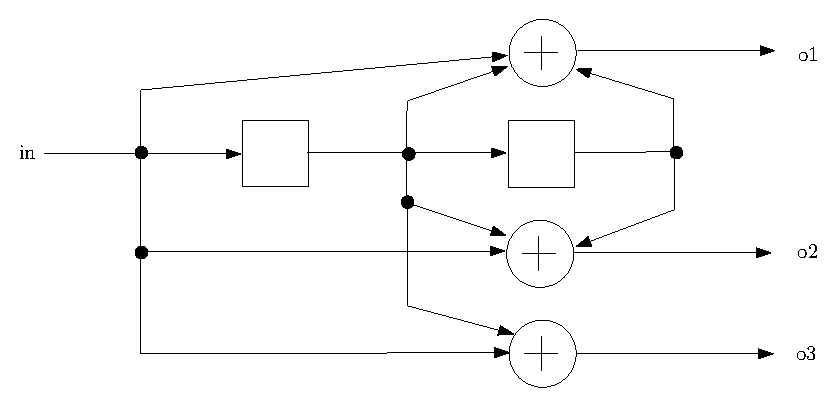
\includegraphics[width=2.5in]{conv_enc.eps}
   \caption{Convolutional encoder. \label{fig:conv_enc} }
\end{figure}


\begin{figure*}
    \psfrag{WER}[Bc][tc][0.8]{WER}
    \psfrag{SNR}[tc][Bc][0.8]{SNR (dB)}
    \psfrag{hard-af-ct----}[cl][cl][0.5]{hard, AF, CT}
    \psfrag{hard-af-eq----}[cl][cl][0.5]{hard, AF, EQ}
    \psfrag{hard-df----}[cl][cl][0.5]{hard, DF}
    \psfrag{soft-af-ct----}[cl][cl][0.5]{soft, AF, CT}
    \psfrag{soft-af-eq----}[cl][cl][0.5]{soft, AF, EQ}
    \psfrag{soft-df----}[cl][cl][0.5]{soft, DF}

\centerline{
    \subfigure[Single Path Relay Network, m=2]{\includegraphics[width=3.25in]{sp_af_df_wer_m2_TU.eps} \label{}}
    \subfigure[Single Path Relay Network, m=4]{\includegraphics[width=3.25in]{sp_af_df_wer_m4_TU.eps} \label{}} \\
}
\centerline{
    \subfigure[Multiple Path Relay Network, m=2]{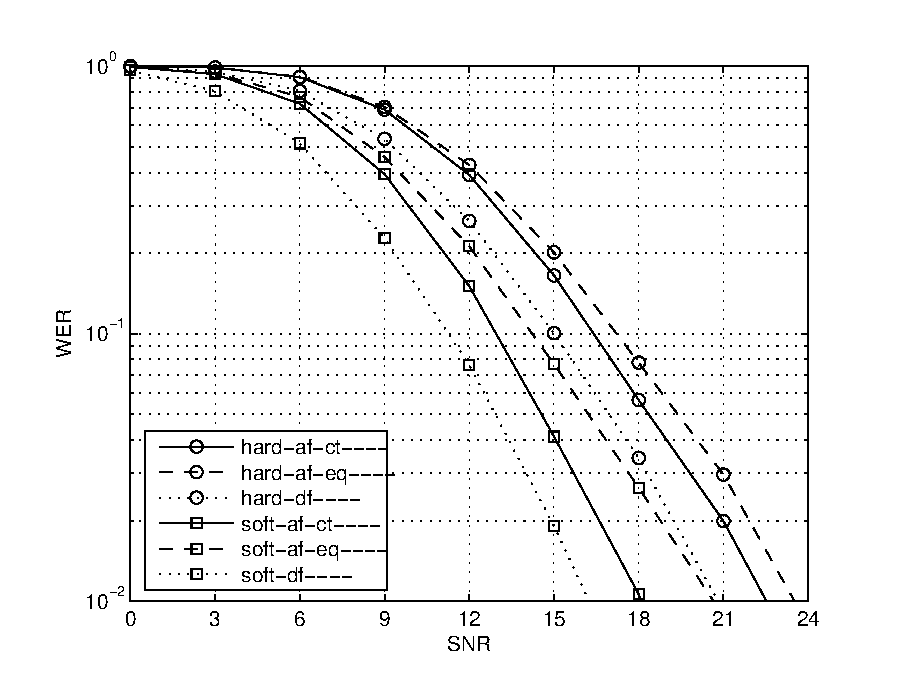
\includegraphics[width=3.25in]{mp_af_df_wer_m2_TU.eps} \label{}}
    \subfigure[Multiple Path Relay Network, m=4]{\includegraphics[width=3.25in]{mp_af_df_wer_m4_TU.eps} \label{}} \\
} \caption{WERs in single path and multiple path relay networks
with TU channels using AF and DF.  $N = 128, m = 2$ and $4$.}
\label{fig:plots}
\end{figure*}

We simulate WERs versus SNR for both the amplify-and-forward and decode-and-forward cases and for both relay networks.  At the transmitter (and at the transmitter structure of a relay using decode-and-forward), each information word contains 83 bits.  Using the convolutional encoder shown in Figure \ref{fig:conv_enc}, the information word is encoded into a 255 bit codeword.  A zero bit is padded at the end to make 256 bits.  The bits are then interleaved and modulated onto $N = 128$ QPSK (quadrature phase shift keying) subcarriers to form one OFDM symbol.  At the receiver (and at the receiver structure of a relay using decode-and-forward), the codeword is recovered (with possible errors) using a matched filter and deinterleaving.  A Viterbi decoder is used to decode the codeword.  Both hard decisions and soft decisions are used.

We consider the $m = 2$ and $4$ relays cases.  We assume that all distances between any two adjacent transceiver nodes are the same.  Therefore, all path loss effects are normalized to 0 dB.  Shadowing is assumed to be log-normally distributed.  That is, the received power gain due to shadowing in dB is a zero-mean Gaussian with variance of 8 dB, which is typical for cellular land mobile applications \cite{book:Stuber01}.  We model frequency selective fading as Typical Urban (TU) channels \cite{book:Stuber01}.  We use an OFDM bandwidth of 800 kHz divided into $N = 128$ equal blocks.  Maintaining OFDM orthogonality, this translates into an OFDM symbol period of $T_s = 160 \:\mu$s.  The simulation results are shown in Figure \ref{fig:plots}.

As shown in the plots, there are significant error rate
performance gains when using decode-and-forward instead of
amplify-and-forward for the single path relay network case.  The
gains are even larger when we increase the distance between the
transmitter and receiver (and thus, add more relays).  The
amplify-and-forward error rates suffer because more channel
distortion and noise enter the system.  The decode-and-forward
error rates suffer only slightly because noise and channel
distortion are eliminated at each relay.  This results in the
large performance gains for $m=4$.  In terms of power allocation
when using amplify-and-forward, CT is the preferable choice since
EQ requires CSI and only results in small performance gains over
CT.

For the multiple path relay network case, the performance gains
resulting from using decode-and-forward instead of
amplify-and-forward diminish as we add more paths between the
transmitter and receiver (and thus, add more relays). This is
because for $m=4$ relays and thus, for 4 paths, the system is
already resistant to noise and channel distortion.  Therefore,
decode-and-forward cannot provide any more significant improvement
over amplify-and-forward.  In such a situation,
amplify-and-forward might be a more attractive choice due to its
lower complexity.  In terms of power allocation when using
amplify-and-forward, CT is the preferable choice because it gives
better performance than EQ and does not require CSI.

As expected, soft decisions give better performance than hard
decisions in Viterbi decoding.


\section{Conlcusions}
\label{sec:conclusions}

In this paper, we investigate cooperation by applying OFDM signals
to a single path relay network and a multiple path relay network.
In particular, we look at the WER performance resulting from such
systems using the amplify-and-forward and decode-and-forward relay
algorithms.  Simulations indicate that decode-and-forward is a
good choice for the single path relay network, because of its
ability to eliminate noise and channel distortion.  For the
multiple path relay network, amplify-and-forward may be the better
choice for its low complexity.

Future research includes investigating relay algorithms other than amplify-and-forward and decode-and-forward in OFDM-based cooperative networks.  For example, hybrid algorithms combining the two can be considered.  That is, depending on the channel conditions, a relay can choose different relay algorithms for different subcarrier symbols in an OFDM signal.  It can amplify-and-forward, decode-and-forward, or even just discard subcarrier symbols.  This in turn leads to more possibilities for relay power allocation.  In this paper, we only investigate the single path relay network and the multiple path relay network.  Other general relay networks need to be considered in the context of OFDM as well.  This will lend more insight into developing a general theoretical framework for OFDM in cooperative relay networks.

\hspace{1cm}

\bibliographystyle{IEEEtran}
\bibliography{IEEEabrv,mybib}

\end{document}
